\documentclass[11pt]{article}
\usepackage[margin=1in]{geometry}
\usepackage{amsmath,amssymb,amsthm,mathrsfs,mathtools}
\usepackage{xcolor}
\usepackage{hyperref}
\usepackage{orcidlink}
\usepackage{tikz}
\hypersetup{colorlinks=true,linkcolor=blue!60!black,citecolor=blue!60!black,urlcolor=blue!60!black}

\newcommand{\Srel}{S^{\mathrm{rel}}}
\newcommand{\Nariai}{Nariai}

\title{\textbf{Does the Area Law Hold on Compact Horizons?}\\ 
Modular Theory and Relative Entropy on the Nariai Horizon}
\author{Brent S. Hartshorn \orcidlink{0009-0004-2853-655X} (\url{brenthartshorn@proton.me})}

\begin{document}
\maketitle

\begin{abstract}
Dorau and Much have shown that the semiclassical Einstein equations follow from Tomita--Takesaki modular theory on a bifurcate Killing horizon, and conversely, given the identification $\Srel = \delta A/4$ of the Araki--Uhlmann relative entropy of a coherent excitation with one quarter of the horizon area variation~\cite{DorauMuch}. We carry the modular part of their construction to the Nariai spacetime $dS_2\times S^2$, where the bifurcation spheres are compact. The relative entropy of coherent excitations is then finite and factorizes exactly into an area-weighted sum of Rindler entropies, with closed-form examples. We also check, rather than derive, the area law: the $s$-wave sector is linearized de~Sitter Jackiw--Teitelboim gravity, whose null equation is the linearized Raychaudhuri equation, and with the modular weight as its Green kernel it gives $|\delta A_{\mathrm{mod}}| = 4G\,\Srel$. This is the converse direction already stated in~\cite{DorauMuch} (the Einstein equations imply the area law); it does not remove the normalization $\Srel = \delta A/4$ from the entropic derivation. We state its limits: the sign of $\delta A$ depends on boundary conditions (retarded data give focusing, teleological data add a memory term); the Nariai instability grows classically at the Hubble rate; and for coherent states positivity of the relative entropy adds nothing to the null energy condition. The coefficient $1/4$ defines Newton's constant and cannot be derived from horizon kinematics; what is checked, by two independent routes (Wald entropy at the horizon, Deser--Tekin charge at infinity), is that in quadratic-curvature gravity and constant-curvature $f(R)$ the same $G_N$ measured at infinity gives $\delta A=4G_N\,\Srel$.
\end{abstract}

\section{Introduction}
\label{sec:intro}

Jacobson's 1995 observation that the Einstein equations can be recovered from the Clausius relation $\delta Q = T\,\delta S$ applied to local Rindler horizons recast gravity as thermodynamics \cite{Jacobson}: an equation of state rather than a fundamental force law. The argument, however, borrowed its entropy from black-hole thermodynamics wholesale, leaving unspecified both the statistical system to which that entropy belongs and the quantum theory in which the heat flux $\delta Q$ is defined. Dorau and Much have recently closed the second gap \cite{DorauMuch}: working entirely within algebraic quantum field theory, they showed that the Araki--Uhlmann relative entropy between a quasifree vacuum state $\omega_0$ and its coherent excitation $\omega_\phi$, evaluated on the horizon algebra of a bifurcate Killing horizon, is
\begin{equation}
\Srel(\omega_0 \,\|\, \omega_\phi)
= -2\pi \int_{\mathcal{H}^{\mathcal{R}}} U \,\langle{:}T_{ab}{:}\rangle_{\omega_\phi}\, \xi^a \xi^b \, dU\, d\mathrm{vol}_{\mathcal{S}},
\label{eq:DM-pivot}
\end{equation}
i.e.\ precisely the boost-energy flux that plays the role of $\delta Q$ in Jacobson's argument \cite{Jacobson}. The heat is no longer thermodynamic bookkeeping; it is a theorem of modular theory. Assuming the Bekenstein--Hawking normalization $\Srel = \delta A/4$ then fixes the coupling of the resulting field equations to $8\pi$, and the semiclassical Einstein equations follow.

This theorem-driven route contrasts with the parallel ``gravity from entropy'' proposal of Bianconi \cite{Bianconi2025,Bianconi2026}, in which the gravitational action is \emph{defined} as a quantum relative entropy between the spacetime metric and a matter-induced metric, and modified Einstein equations follow by variation --- at the price of truncations (a reduced Dirac--K\"ahler field content, an auxiliary-field reformulation) whose consistency with the general theory is not demonstrated. The route pursued here is complementary: no new action and no truncation, but modular theory on an exact solution, in which every quantity is finite and each step is either taken from the literature, computed here, or flagged as an input. The two programs converge on the question both must ultimately answer: what the entropy that sources gravity is an entropy \emph{of}.

Dorau and Much state their result as a biconditional: assuming $\Srel = \delta A/4$ one recovers the semiclassical Einstein equations, and conversely \cite{DorauMuch}. What the derivation does not supply, and does not claim to supply, is a reason for that normalization. The relative entropy itself is unambiguous --- it is the distinguishability of a coherent excitation from the vacuum, and Bianconi's construction is likewise explicit about its two arguments, the spacetime metric and the matter-induced metric \cite{Bianconi2025} --- but the factor $1/4$ imports a statement about gravitational microstates from black-hole thermodynamics. In Ref.~\cite{DorauMuch} the metric perturbation that realizes an area variation is an ansatz; the substantive assumption is the proportionality $\delta A\propto\Srel$ with the Bekenstein--Hawking coefficient.

This paper does not remove that assumption. The normalization $\Srel=\delta A/4$, the Einstein equations and the area response are equivalent statements in the biconditional of Ref.~\cite{DorauMuch}, and the coefficient $1/4$ in the entropy and the $8\pi$ of the reduced action are the same Newton constant. What we do is (i) carry the modular computation to Nariai, where the cross-sections are compact and every transverse integral is finite; (ii) check on this background that the $s$-wave dynamics is consistent with the normalization, which is the converse direction of Ref.~\cite{DorauMuch}; and (iii) record what Nariai does and does not add. Compactness does not help the entropy itself: the Araki--Uhlmann entropy of a coherent excitation equals an area \emph{variation}, which is well defined when the cross-section is non-compact, as the Rindler case and the analysis of Ref.~\cite{DAngelo} show. Nothing below turns on replacing $\delta A$ by $A$.

The geometry is $dS_2 \times S^2$, the degenerate limit of the Schwarzschild--de~Sitter family in which the black-hole and cosmological horizons have equal radius $r = 1/\sqrt{\Lambda}$ \cite{Nariai}. Its dS$_2$ static patch has \emph{two} Killing horizons, the black-hole and cosmological horizons of the parent family, which are distinct bifurcate Killing horizons with their own bifurcation spheres and, at this point, equal surface gravity. The modular algebra of this paper lives on one of them. The normalization of the Killing field is fixed by the geometry through the Bousso--Hawking prescription \cite{BoussoHawking}. De~Sitter space itself already offers compact cross-sections, a geometric normalization and an invariant state, and its entropy--area law was derived by modular theory in Ref.~\cite{DAngelo}; what Nariai adds is an \emph{equilibrium of two horizons at one temperature}, which generic Schwarzschild--de~Sitter lacks, together with a background that is unstable. We do not claim it is the only such arena. The instability matters for the modular construction, which presupposes a fixed Killing horizon, and Section~\ref{sec:timescales} states the resulting window of validity.

\paragraph{What is taken from the literature, and what is new.} The scaling-limit two-point function and the modular structure on a bifurcate Killing horizon are due to Kay and Wald \cite{KayWald} and to Summers and Verch \cite{SummersVerch}; the formula for the relative entropy of a coherent excitation, and its identification with the boost-energy flux, are due to Kurpicz, Pinamonti and Verch \cite{KPV} and to Dorau and Much \cite{DorauMuch}. Sections~\ref{sec:algebra}--\ref{sec:entropy} apply their results to \Nariai{}, and several displayed equations coincide with those of Ref.~\cite{DorauMuch} (we mark this where it occurs). The dimensional reduction of the throat to de~Sitter JT gravity is standard \cite{MertensTuriaci}. What is specific to this paper is modest: the finite factorization \eqref{eq:factorized} and the closed-form family of Section~\ref{sec:example}; the consistency check of Section~\ref{sec:JT}, including the correct sign of the dilaton equation, the dependence on boundary conditions, and the zero modes; the statement of the window of validity of the static modular description in Section~\ref{sec:timescales}; and the scope remark that the coupling is Einstein's (Section~\ref{sec:JT}).

The Dorau--Much quantity \eqref{eq:DM-pivot} is not a von Neumann entropy of a hidden substrate; it is a \emph{relative} entropy, the information-theoretic distinguishability of the realized state $\omega_\phi$ from the \emph{counterfactual vacuum} $\omega_0$. It measures, in the only sense the algebraic theory makes available, how
much the world that happened differs from the world that did not.


% ====================================================================
\section{The \Nariai{} Geometry and its Bifurcate Killing Horizon}
\label{sec:geometry}

Throughout we use units $G = \hbar = c = 1$, so that areas, entropies and energies are measured in Planck units and the Einstein coupling appears as $8\pi$.

\subsection{The Schwarzschild--de Sitter family and its degenerate limit}

The Schwarzschild--de Sitter (SdS) family in four dimensions,
\begin{equation}
ds^2 = -f(r)\,dt^2 + \frac{dr^2}{f(r)} + r^2\, d\Omega^2,
\qquad
f(r) = 1 - \frac{2M}{r} - \frac{\Lambda r^2}{3},
\label{eq:SdS}
\end{equation}
possesses, for $0 < 9\Lambda M^2 < 1$, two positive roots of $f$: the black-hole horizon $r_b$ and the cosmological horizon $r_c > r_b$. Their surface gravities,
\begin{equation}
\kappa_{b,c} = \tfrac{1}{2}\,|f'(r_{b,c})|,
\end{equation}
are unequal for any nondegenerate member of the family. This inequality is why generic SdS is a poor arena for the algebraic construction of Ref.~\cite{DorauMuch}: the two horizons define inequivalent notions of thermal equilibrium, no globally regular Killing-invariant Hadamard state exists on the full extension (the obstruction identified by Kay and Wald~\cite{KayWald}), and any horizon-by-horizon treatment inherits an ambiguity in the reference state --- an ambiguity that the common remedy of partitioning SdS by timelike boundaries \cite{Rusalev} makes explicit rather than removes.

The degenerate limit removes the obstruction. As $9\Lambda M^2 \to 1$ the two roots merge at
\begin{equation}
r_b, r_c \;\to\; r_\star = \frac{1}{\sqrt{\Lambda}} = 3M,
\end{equation}
and the region between the horizons acquires a finite invariant description. Following the Ginsparg--Perry procedure~\cite{GinspargPerry}, set
\begin{equation}
9\Lambda M^2 = 1 - 3\varepsilon^2, \qquad 0 \le \varepsilon \ll 1,
\end{equation}
and introduce coordinates $(\psi, \chi)$ adapted to the near-degenerate throat,
\begin{equation}
t = \frac{\psi}{\varepsilon\sqrt{\Lambda}},
\qquad
r = \frac{1}{\sqrt{\Lambda}}\left(1 - \varepsilon\cos\chi \right) + \mathcal{O}(\varepsilon^2).
\end{equation}
In the limit $\varepsilon \to 0$ the metric \eqref{eq:SdS} becomes the \Nariai{} spacetime~\cite{Nariai}
\begin{equation}
ds^2 = \frac{1}{\Lambda}\left(-\sin^2\!\chi \, d\psi^2 + d\chi^2\right) + \frac{1}{\Lambda}\, d\Omega^2 ,
\label{eq:nariai-global}
\end{equation}
the direct product $dS_2 \times S^2$ of a two-dimensional de~Sitter factor and a round two-sphere, both of curvature radius $1/\sqrt{\Lambda}$. Unlike the near-horizon limits of asymptotically flat extremal black holes, \eqref{eq:nariai-global} is an exact solution of the Einstein equations with cosmological constant $\Lambda$, and it is the member of the SdS family at which the black-hole and cosmological horizons have equal surface gravity. De~Sitter space itself also admits a global bifurcate Killing horizon with a single surface gravity (it is the $M=0$ member), so equal surface gravity is not unique to Nariai; what is specific is that two distinct horizons are in equilibrium at one temperature.


\begin{figure}[t]
\centering
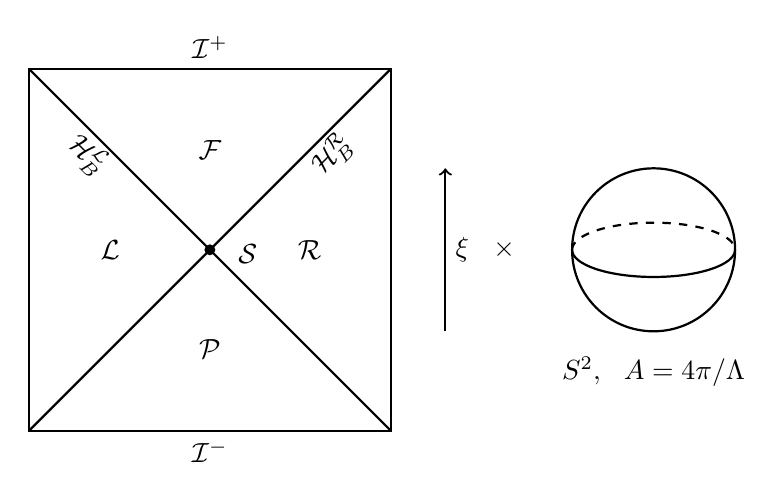
\begin{tikzpicture}[scale=1.15]
  % the dS_2 factor: a Penrose square with the bifurcate horizon
  \draw[thick] (-2,-2) rectangle (2,2);
  \draw[thick] (-2,-2) -- (2,2);
  \draw[thick] (-2,2) -- (2,-2);
  \node at (0,0) [circle,fill,inner sep=1.4pt] {};
  \node at (0.42,-0.05) {$\mathcal{S}$};
  \node at (1.1,0) {$\mathcal{R}$};
  \node at (-1.1,0) {$\mathcal{L}$};
  \node at (0,1.1) {$\mathcal{F}$};
  \node at (0,-1.1) {$\mathcal{P}$};
  \node[above] at (0,2) {$\mathcal{I}^+$};
  \node[below] at (0,-2) {$\mathcal{I}^-$};
  \node[rotate=45] at (1.35,1.05) {$\mathcal{H}^{\mathcal{R}}_B$};
  \node[rotate=-45] at (-1.35,1.05) {$\mathcal{H}^{\mathcal{L}}_B$};
  \draw[->,thick] (2.6,-0.9) -- (2.6,0.9) node[midway,right] {$\xi$};
  % the transverse sphere
  \draw[thick] (4.9,0) circle (0.9);
  \draw[thick] (4.0,0) arc (180:360:0.9 and 0.3);
  \draw[thick,dashed] (4.0,0) arc (180:0:0.9 and 0.3);
  \node at (4.9,-1.35) {$S^2,\ \ A = 4\pi/\Lambda$};
  \node at (3.25,0) {$\times$};
\end{tikzpicture}
\caption{The \Nariai{} geometry $dS_2 \times S^2$. Left: the conformal diagram of the $dS_2$ factor. The two null lines are the bifurcate Killing horizon, meeting at the bifurcation surface $\mathcal{S}$; $\mathcal{R}$ and $\mathcal{L}$ are the two static patches, in which the Killing field $\xi$ is timelike, and $\mathcal{F}$, $\mathcal{P}$ their future and past. The horizon algebra of Section~\ref{sec:algebra} lives on $\mathcal{H}^{\mathcal{R}}_B=\{V=0,\,U<0\}$, which is the \emph{past} horizon of the static patch $\mathcal R$. The $dS_2$ static patch has two such horizons (the black-hole and cosmological horizons of the parent family); only one is drawn. Right: every point of the diagram is a round two-sphere of radius $1/\sqrt{\Lambda}$; the bifurcation surface is compact, with area $4\pi/\Lambda$. In generic Schwarzschild--de~Sitter the two null lines carry different surface gravities; in the degenerate limit they are equal, which is what makes a single Killing flow and a global KMS state available.}
\label{fig:nariai}
\end{figure}

\subsection{Static patch, horizon structure, and the normalization of the Killing field}
The geometry is drawn in Figure~\ref{fig:nariai}. 
Substituting $\rho = \Lambda^{-1/2}\cos\chi$ and $\tau = \Lambda^{-1/2}\psi$ brings the $dS_2$ factor to static form,
\begin{equation}
ds^2 = -\big(1-\Lambda\rho^2\big)\,d\tau^2 + \frac{d\rho^2}{1-\Lambda\rho^2} + \frac{1}{\Lambda}\,d\Omega^2 ,
\label{eq:nariai-static}
\end{equation}
with Killing field $\xi = \partial_\tau$ and Killing horizons at $\rho = \pm \Lambda^{-1/2}$. The surface gravity of $\xi$ is
\begin{equation}
\kappa = \sqrt{\Lambda}\,,
\qquad
T = \frac{\kappa}{2\pi} = \frac{\sqrt{\Lambda}}{2\pi}\,,
\label{eq:temperature}
\end{equation}
which is the Bousso--Hawking temperature of the degenerate solution~\cite{BoussoHawking}. Two remarks on normalization are essential, because this is the hinge on which the modular theory of Section~\ref{sec:algebra} turns. First, the limit must be taken in the rescaled time $\psi$, not in the SdS time $t$: the surface gravities $\kappa_{b,c}$ of the parent family both vanish as $\varepsilon \to 0$, and a construction anchored to $\partial_t$ would see zero temperature. The rescaling $t = \psi/(\varepsilon\sqrt{\Lambda})$ is the Bousso--Hawking prescription of normalizing the generator with respect to the inertial observer suspended between the horizons. Second --- and this is where \Nariai{} improves on the Rindler wedge --- the normalization is \emph{not} ambiguous. The Rindler boost generator admits arbitrary rescaling, correspondingly rescaling the Unruh temperature, a freedom Ref.~\cite{DorauMuch} notes as an intrinsic limitation of the local construction. On \Nariai{} the geometry itself supplies the scale: the Killing field in \eqref{eq:nariai-static} is fixed (up to sign) by unit normalization on the central geodesic $\rho = 0$, and the temperature \eqref{eq:temperature} is an invariant of the solution.

With $\rho_*$ the tortoise coordinate of \eqref{eq:nariai-static} and $u,v = \tau \mp \rho_*$, the affine (Kruskal-type) coordinates
\begin{equation}
U = -\frac{1}{\kappa}\,e^{-\kappa u},
\qquad
V = +\frac{1}{\kappa}\,e^{+\kappa v},
\end{equation}
extend the static patch to the full square Penrose diagram of $dS_2$, every point of which carries the sphere $S^2_{1/\sqrt{\Lambda}}$. The global null hypersurfaces $\mathcal{H}_B = \{V = 0\}$ and $\mathcal{H}_A = \{U = 0\}$, generated by the flow of $\xi$, intersect on the bifurcation surface
\begin{equation}
\mathcal{S} = S^2_{1/\sqrt{\Lambda}},
\qquad
A(\mathcal{S}) = \frac{4\pi}{\Lambda}\,,
\label{eq:area}
\end{equation}
a \emph{compact} two-sphere. The pair $(\mathcal{H}_A, \mathcal{H}_B)$ is a bifurcate Killing horizon in the exact sense of Kay and Wald~\cite{KayWald}, realized globally rather than as a local approximation, with cross-sectional volume element $d\mathrm{vol}_{\mathcal{S}} = \Lambda^{-1}\sin\theta\, d\theta\, d\varphi$ integrating to the finite total \eqref{eq:area}. Every transverse integral in Sections~\ref{sec:algebra} and~\ref{sec:entropy} is therefore finite from the outset, and the associated horizon entropy
\begin{equation}
S_{\mathrm{N}} = \frac{A(\mathcal{S})}{4} = \frac{\pi}{\Lambda}
\label{eq:Smax}
\end{equation}
is finite. It is \emph{not} the maximal horizon entropy in the SdS family at fixed $\Lambda$: pure de~Sitter space ($M=0$) has cosmological-horizon area $12\pi/\Lambda$ and entropy $3\pi/\Lambda$, and along the family the cosmological horizon area decreases monotonically to $4\pi/\Lambda$ while the black-hole horizon area increases from $0$ to $4\pi/\Lambda$. Nariai is the maximal black-hole horizon and the minimal cosmological horizon (verified numerically in \texttt{check\_referee\_points.py}).

\subsection{Global hyperbolicity and the Euclidean section}

Two further structural facts prepare the ground. First, $dS_2 \times S^2$ is globally hyperbolic (a product of globally hyperbolic $dS_2$ with a compact Riemannian factor), so the algebraic quantization of a Klein--Gordon field proceeds without the causal subtleties of generic SdS. Second, the Euclidean section obtained by $\psi \to -i\psi_E$ is the round product $S^2 \times S^2$, compact and everywhere regular, with thermal periodicity $\psi_E \sim \psi_E + 2\pi$ built into the geometry. For a field of mass $m>0$ there is consequently a distinguished Hartle--Hawking-type state $\omega_0$ (for $m=0$ the $S^2\times S^2$ section has a constant zero mode and no Euclidean vacuum exists): obtained by analytic continuation from the regular Euclidean section, invariant under the Killing flow, Hadamard, and KMS at the temperature \eqref{eq:temperature}. For nondegenerate SdS no such globally regular equilibrium state exists --- the two unequal temperatures forbid it --- so the degeneracy of \Nariai{} is not a curiosity we tolerate but the very feature that makes a preferred global vacuum available. It is this $\omega_0$ that plays the role of the reference state: the ``unrealized'' side of the relative entropy.

\subsection{The Nariai instability and the window of validity of the modular description}
\label{sec:timescales}

Tomita--Takesaki theory itself requires no geometry: a von Neumann algebra with a cyclic separating vector suffices. What requires geometry is the \emph{identification} of the modular flow with the Killing flow --- the Bisognano--Wichmann property and its curved-space form for bifurcate Killing horizons \cite{Sewell,KayWald} --- and it is that identification, on which the modular Hamiltonian of Section~\ref{sec:modularH} and hence the Araki--Uhlmann entropy rest, that presupposes a fixed bifurcate Killing horizon carrying an invariant KMS state $\omega_0$. But the \Nariai{} background is the unstable saddle governing the semiclassical decay of de~Sitter space \cite{GinspargPerry,BoussoHawking}. In what sense, then, is a \emph{static} modular Hamiltonian available?

\paragraph{The instability is classical in its growth.} Within the static family \eqref{eq:SdS} the parameter $\varepsilon$ labels exactly static solutions, but that is the view from a single static patch. Linear perturbations of $dS_2\times S^2$ are not static. In global $dS_2$ with metric $\Lambda^{-1}(-dT^2+\cosh^2T\,d\theta^2)$ the homogeneous solutions of the linearized $s$-wave dilaton equation (Eq.~\eqref{eq:JT-eom} below) are
\begin{equation}
\phi_{\mathrm{dil}} \in \mathrm{span}\{\sinh T,\ \cosh T\cos\theta,\ \cosh T\sin\theta\}\,,
\label{eq:zero-modes}
\end{equation}
which grow as $e^{\sqrt{\Lambda}\,\tau}$ in proper time $\tau = T/\sqrt\Lambda$. The Ginsparg--Perry deformation $\varepsilon\cos\chi$ is one of them. The growth rate is therefore of order $\kappa=\sqrt\Lambda$, \emph{not} $\kappa/S_{\mathrm N}$. This is the classical, Hubble-rate growth of Nariai perturbations known from the literature \cite{Bousso1998}; $\hbar$ enters only through the amplitude of the seed supplied by quantum fluctuations. The check that \eqref{eq:zero-modes} solves the dilaton equation, and that it does so only with the sign of the $\Lambda$ term given in Eq.~\eqref{eq:JT-eom}, is performed symbolically in the repository (\texttt{check\_referee\_points.py}).

\paragraph{The window.} The modular time is $t_{\mathrm{mod}}=\beta=2\pi/\kappa$. A seed of amplitude $\varepsilon_0$ reaches order one after a time of order $\kappa^{-1}\ln(1/\varepsilon_0)$; with a quantum seed, $\varepsilon_0\sim \hbar^{1/2}$ in units of the curvature radius, i.e.\ $\varepsilon_0\sim S_{\mathrm N}^{-1/2}$ (a parametric estimate, not a derived amplitude), this is at most of order $\kappa^{-1}\ln S_{\mathrm N}$. The estimate enters only through its logarithm: for a seed $\varepsilon_0\sim S_{\mathrm N}^{-p}$ the time is $p\,\kappa^{-1}\ln S_{\mathrm N}$, so any power law in $S_{\mathrm N}$ gives a window of order $\ln S_{\mathrm N}$ (for the observed $\Lambda$, $140$, $281$, $562$ for $p=\tfrac12,1,2$). What this does not control is a seed that is not a power of $S_{\mathrm N}$, which would require a computation of the quantum fluctuation amplitude of the growing mode that is not attempted here. It follows that the static description is controlled for excitations whose support $\Delta u$ in boost time satisfies
\begin{equation}
\kappa\,\Delta u \;\ll\; \ln S_{\mathrm N}\,,
\label{eq:hierarchy}
\end{equation}
that is, the relative deformation of the background accumulated over the support is $\varepsilon_0\,e^{\kappa\Delta u}\ll1$. For the observed $\Lambda$, $\ln S_{\mathrm N}$ is a few hundred, so a single-modular-period event ($\kappa\Delta u=\mathcal O(1)$, as in Section~\ref{sec:example}) sits comfortably inside the window, but the window is logarithmic in $S_{\mathrm N}$, not a power. In particular the instability does not proceed at the rate $\kappa/S_{\mathrm N}$, and a ratio $t_{\mathrm{inst}}/t_{\mathrm{mod}}\sim S_{\mathrm N}$ is not a hierarchy that protects the construction. The nucleation channel through the $S^2\times S^2$ instanton, $\propto e^{-S_{\mathrm N}}$ \cite{GinspargPerry}, is a separate and much slower process.

\paragraph{Consequences.} (a) Sections~\ref{sec:algebra} and \ref{sec:entropy} are exact statements about the fixed background; they are zeroth order in the deformation, and corrections from the growing mode are of relative order $\varepsilon_0\,e^{\kappa\Delta u}$ as above. (b) The entropy formula depends on the background through two structures, the universal Kay--Wald kernel \eqref{eq:scaling-limit} and the transverse measure, so it is insensitive to a slow drift but not to an exponentially growing one outside the window. (c) Outside the window, or near the branch endpoints, no static modular Hamiltonian is available and the present construction makes no claim; the memory mode of Section~\ref{sec:JT} is a classical solution whose coefficient is set by the absorbed flux, and it does not evolve at a rate $\kappa/S_{\mathrm N}$ either.

\section{Horizon Algebra and Modular Structure on \Nariai{}}
\label{sec:algebra}

\noindent\emph{Overlap with Ref.~\cite{DorauMuch}.} The scaling-limit kernel \eqref{eq:scaling-limit}, the symplectic form \eqref{eq:symplectic}, the Weyl algebra and quasifree state, the modular dilations \eqref{eq:dilations}, the Araki computation \eqref{eq:araki-formula}--\eqref{eq:Srel-nariai}, the pivot identity \eqref{eq:pivot-nariai} and the ansatz \eqref{eq:perturbation} coincide with the corresponding equations of Ref.~\cite{DorauMuch} (their Eqs.~(3), (5)--(13), (19), (20)), transcribed to the compact horizon. The only changes are the finite transverse measure and the discrete harmonic decomposition.

\subsection{Field content and dimensional reduction}

Let $\Phi$ be a real, minimally coupled Klein--Gordon field of mass $m$ on $dS_2 \times S^2$. The product structure separates the wave operator,
\begin{equation}
\square_g = \square_{dS_2} + \Lambda\, \Delta_{S^2},
\end{equation}
so expanding in spherical harmonics, $\Phi = \sum_{\ell m} \varphi_{\ell m}(\psi,\chi)\, Y_{\ell m}(\theta,\varphi)$, reduces the theory to an infinite tower of two-dimensional fields $\varphi_{\ell m}$ on $dS_2$ with effective masses
\begin{equation}
m_\ell^2 = \underbrace{m^2}_{\text{bare mass}} + \underbrace{\Lambda\,\ell(\ell+1)}_{\substack{\text{Kaluza--Klein mass}\\ \text{from the compact } S^2}}, \qquad \ell = 0, 1, 2, \dots
\label{eq:tower}
\end{equation}
The scaling limit below is insensitive to the tower, but \eqref{eq:tower} does two jobs. It exhibits the compactness of $\mathcal{S}$ as a physical regulator --- the transverse degrees of freedom are a discrete tower rather than a continuum, which is ultimately why the entropy integrals of Section~\ref{sec:entropy} converge without subtraction --- and it explains \emph{why} the $s$-wave sector $\ell = 0$ dominates near-horizon physics. On the $dS_2$ factor, of Hubble rate $\sqrt{\Lambda}$, every $\ell \ge 1$ member of \eqref{eq:tower} is a heavy, principal-series field, $m_\ell^2/\Lambda \ge 2 > \tfrac{1}{4}$, with $\nu_\ell = \sqrt{\ell(\ell+1) + m^2/\Lambda - \tfrac{1}{4}}$; its static-patch correlators decay rapidly and its thermal excitation is Boltzmann-suppressed as $e^{-\pi\nu_\ell} \sim e^{-\pi\ell}$. Each successive harmonic is suppressed in the bulk of the static patch, which is why the $s$-wave sector governs the dilaton dynamics of Section~\ref{sec:JT}. This does \emph{not} suppress higher harmonics on the horizon algebra: the horizon kernel \eqref{eq:scaling-limit} and the entropy \eqref{eq:factorized} are $\ell$-blind, so every harmonic contributes to $\Srel$ at full weight.

\subsection{The scaling-limit two-point function on a compact horizon}

By the Kay--Wald analysis~\cite{KayWald}, the restriction of any Killing-flow-invariant Hadamard state to $\mathcal{H}_B$ possesses the universal scaling-limit two-point function; on \Nariai{} it takes exactly the form of Ref.~\cite{DorauMuch},
\begin{equation}
\Lambda_2(\phi, \psi)
= -\frac{1}{\pi} \int
\frac{\phi(U, s)\, \psi(U', s)}{(U - U' - i0^+)^2}\;
dU\, dU'\, d\mathrm{vol}_{\mathcal{S}},
\label{eq:scaling-limit}
\end{equation}
for $\phi, \psi \in C^\infty_c(\mathcal{H}_B)$, where now $s = (\theta,\varphi)$ ranges over the \emph{compact} bifurcation sphere and $d\mathrm{vol}_{\mathcal{S}} = \Lambda^{-1} \sin\theta\, d\theta\, d\varphi$. Three properties deserve emphasis.

\begin{enumerate}
\item \emph{Universality survives compactification.} The kernel in $U$ is the same conformal kernel as in the Rindler and Schwarzschild cases: the scaling limit forgets the mass tower \eqref{eq:tower} and the $dS_2$ curvature, retaining only the null-line conformal structure and the transverse measure. The horizon theory is effectively a chiral theory in $U$ fibered over $\mathcal{S}$ --- but the fiber integral is now finite.

\item \emph{The reference state is canonical.} On the Rindler horizon the state whose restriction yields \eqref{eq:scaling-limit} is the Minkowski vacuum; on \Nariai{} it is the Euclidean state $\omega_0$ of Section~\ref{sec:geometry}, distinguished by regularity on $S^2\times S^2$ and KMS at $\beta = 2\pi/\sqrt{\Lambda}$ with respect to the projected Killing flow.

\item \emph{The symplectic structure is finite.} For compactly supported test functions it is finite whether or not $\mathcal{S}$ is compact; what compactness of $\mathcal{S}$ gives is that the transverse decomposition is a discrete sum and that transversally homogeneous data have finite norm. The imaginary part of \eqref{eq:scaling-limit} equips $C^\infty_c(\mathcal{H}_B^{\mathcal{R}})$ with the symplectic form
\begin{equation}
\sigma(\phi,\psi)
= \int \big(\phi\,\partial_U \psi - \psi\,\partial_U \phi\big)\, dU\, d\mathrm{vol}_{\mathcal{S}},
\label{eq:symplectic}
\end{equation}
finite for transversally homogeneous ($\ell = 0$) data because the total area $4\pi/\Lambda$ is finite; on the Rindler horizon such data are not admissible.

\end{enumerate}


\subsection{Weyl algebra, modular dilations, and the KMS structure}

The horizon von Neumann algebra now proceeds verbatim along Ref.~\cite{DorauMuch} and the modular analysis of Summers and Verch~\cite{SummersVerch}. Over $\big(C_c^\infty(\mathcal{H}_B^{\mathcal{R}}), \sigma\big)$ one builds the Weyl algebra $\mathscr{W}_{\mathcal{R}}$, generated by unitaries $W(\phi)$ satisfying
\begin{equation}
W(\phi)^\dagger = W(-\phi),
\qquad
W(\phi) W(\psi) = e^{-\frac{i}{2}\sigma(\phi,\psi)}\, W(\phi+\psi),
\end{equation}
represents it in the GNS representation $(\mathscr{H}_0, \pi_0, \Omega_0)$ of the quasifree state
\begin{equation}
\omega_0\big(W(\psi)\big) = e^{-\frac{1}{2}\Lambda_2(\psi,\psi)},
\end{equation}
and takes the double commutant $\mathscr{N}_{\mathcal{R}} = \pi_0(\mathscr{W}_{\mathcal{R}})''$. The vector $\Omega_0$ is cyclic and separating for $\mathscr{N}_{\mathcal{R}}$, and the associated Tomita--Takesaki modular group acts geometrically as affine dilations of the horizon generators,
\begin{equation}
\Delta_{\mathcal{R}}^{it} = \mathfrak{D}_{-2\pi t}:
\qquad
\phi(U, s) \;\longmapsto\; \phi\big(e^{-2\pi t}\, U,\; s\big),
\label{eq:dilations}
\end{equation}
leaving the compact transverse coordinate $s$ untouched; the orientation of the flow (contraction of $\mathcal{H}_B^{\mathcal{R}}$, the past horizon of $\mathcal R$ on which $U<0$, toward the bifurcation surface as $t \to +\infty$) is fixed by the KMS condition, as follows. For test functions supported on $U<0$ the function $F(t)=\langle\Omega_0,A\,\sigma_t(B)\,\Omega_0\rangle$ built from \eqref{eq:scaling-limit} and the dilation $U'\mapsto \lambda U'$, $\lambda=e^{2\pi t}$, is a meromorphic function of $\lambda$ whose only singularity is the positive real ray $\lambda=|U|/|U'|$. The boundary value of the kernel at real $t$ is the one with $-i0$, i.e.\ $\lambda$ just \emph{below} the ray. Continuing to $\operatorname{Im}t\to-1$ turns $\lambda$ through the angle $-2\pi$ without crossing the ray, so $F$ is analytic in $-1<\operatorname{Im}t<0$ and arrives at the ray from \emph{above}, which is the kernel with $+i0$, i.e.\ the opposite operator ordering $\langle\sigma_t(B)A\rangle$: exactly the Tomita--Takesaki strip condition. The opposite orientation $\lambda=e^{-2\pi t}$ interchanges the two boundary values and violates it. This is not a convention, because the two orderings differ by the symplectic form, which is non-zero; the check is performed numerically, with the commutator also obtained by a second route, in \texttt{check\_open\_items.py}. The sign convention of the orientation relative to Eq.~(4) of Ref.~\cite{DorauMuch} has not been compared term by term, and the derivation rests on the positive-energy ($-i0$) prescription of the Kay--Wald kernel with respect to $U$. This is the Bisognano--Wichmann property in its bifurcate-horizon generalization: it delivers, as a theorem rather than an input, the identification of the geometric Killing flow with the modular flow of $(\mathscr{N}_{\mathcal{R}}, \Omega_0)$ at the Bousso--Hawking temperature \eqref{eq:temperature}.

\subsection{The modular Hamiltonian in explicit form}
\label{sec:modularH}

For the computations of Section~\ref{sec:entropy} it is worth descending to explicit formulas. Differentiating \eqref{eq:dilations} at $t=0$, the generator $K = -\ln \Delta_{\mathcal{R}}$ acts on horizon data as $2\pi\, U \partial_U$, and its second-quantized form on the full horizon is the modular-weighted flux operator
\begin{equation}
K \;=\; -\ln \Delta_{\mathcal{R}}
\;=\; \underbrace{2\pi \int_{\mathcal{S}} d\mathrm{vol}_{\mathcal{S}} \int_{-\infty}^{0} (-U)\, {:}T_{UU}(U,s){:}\; dU}_{\displaystyle K_{\mathcal{R}}\;(\text{right-portion boost energy})}
\;-\;
\underbrace{2\pi \int_{\mathcal{S}} d\mathrm{vol}_{\mathcal{S}} \int_{0}^{\infty} U\, {:}T_{UU}(U,s){:}\; dU}_{\displaystyle K_{\mathcal{L}}\;(\text{left portion})}\,,
\label{eq:modularH}
\end{equation}
with $K_{\mathcal{R}}$ generating the dilations \eqref{eq:dilations} on $\mathcal{H}_B^{\mathcal{R}}$. The one-sided $K_{\mathcal R}$ is at best a quadratic form, not an operator affiliated with $\mathscr N_{\mathcal R}$; only its expectation values in coherent states are used. Both integrals are individually finite in expectation on Hadamard excitations of $\omega_0$: the modular weight $|U|$ vanishes linearly at the bifurcation surface while the normal-ordered flux is integrable along the generators, and the transverse integral is bounded by the total area \eqref{eq:area}. On the Rindler horizon the same expression exists only as a formal density in the transverse plane; on \Nariai{} it is an honest (unbounded, self-adjoint) operator expression with finite state-dependent expectation values.

Equation \eqref{eq:modularH} is the null-coordinate face of the modular Hamiltonian. Its static face follows from the Bisognano--Wichmann identification: $K_{\mathcal{R}} = \beta\, H_\xi$ with $\beta = 2\pi/\sqrt{\Lambda}$, where $H_\xi$ is the Killing energy on a static slice $\Sigma_\tau$ of \eqref{eq:nariai-static}. With $\sqrt{h}\, d\rho\, d\Omega = (1-\Lambda\rho^2)^{-1/2}\, \Lambda^{-1} \sin\theta\, d\rho\, d\theta\, d\varphi$ and $n^a = (1-\Lambda\rho^2)^{-1/2}\, \delta^a_{\;\tau}$,
\begin{equation}
K_{\mathcal{R}} \;=\; \frac{2\pi}{\sqrt{\Lambda}}\; H_\xi\,,
\qquad
H_\xi
= \int_{\Sigma_\tau} T_{ab}\, \xi^a n^b\, d\Sigma
= \frac{1}{\Lambda} \int_{S^2} d\Omega \int_{-1/\sqrt{\Lambda}}^{\,1/\sqrt{\Lambda}}
\frac{{:}T_{\tau\tau}(\rho, s){:}}{1 - \Lambda \rho^2}\; d\rho\,,
\label{eq:KillingH}
\end{equation}
the energy flux integrated across the full throat. The two ends of the throat are the two \emph{distinct} Killing horizons (black-hole and cosmological), and deforming $\Sigma_\tau$ to the horizon reaches both, whereas the null face \eqref{eq:modularH} uses only $\mathcal H_B^{\mathcal R}$. The two faces therefore agree only for excitations whose flux crosses a single horizon; the computations below are for such excitations, and the Killing energy $E_\xi$ used in the Clausius relation of Section~\ref{sec:example} is understood as this one-horizon restriction. The apparent divergence of the measure at $\rho \to \pm 1/\sqrt{\Lambda}$ is compensated for Hadamard states by $T_{\tau\tau} \propto (1-\Lambda\rho^2)$; and because the geometry fixes the normalization of $\xi$ (Section~\ref{sec:geometry}), the Killing energy \eqref{eq:KillingH} carries no rescaling ambiguity. The two faces \eqref{eq:modularH} and \eqref{eq:KillingH} are related on-shell by deforming $\Sigma_\tau$ to the horizon; the boost-Jacobian identity $(-U)\,(\partial_U\chi)^2\,dU = \kappa^{-1}(\partial_u\chi)^2\,du$, with $U = -\kappa^{-1}e^{-\kappa u}$ the boost time on the horizon, is precisely this deformation in coordinates. For coherent states Araki's formula gives directly (no von Neumann entropy difference is involved, since $\mathscr N_{\mathcal R}$ is of type III) the expectation-value shift of \eqref{eq:modularH},
\begin{equation}
\Srel(\omega_0\,\|\,\omega) \;=\; \langle K_{\mathcal{R}} \rangle_{\omega} - \langle K_{\mathcal{R}} \rangle_{\omega_0}\,,
\label{eq:Srel-K}
\end{equation}
which is the form in which the explicit computations below will be organized.

Coherent excitations are defined as in the flat case: for $\phi \in C_c^\infty(\mathcal{H}_B^{\mathcal{R}})$,
\begin{equation}
\omega_\phi\big(W(\psi)\big) = \omega_0\big(W(\phi)^\dagger\, W(\psi)\, W(\phi)\big),
\qquad
\Omega_\phi = e^{i\Phi(\phi)}\,\Omega_0 .
\label{eq:coherent}
\end{equation}
Physically, $\omega_\phi$ describes the \Nariai{} equilibrium disturbed by a classical pulse of scalar radiation crossing the horizon --- the minimal ``event'' against the background of the eventless vacuum. With the algebra, the modular geometry \eqref{eq:dilations}, and the state pair $(\omega_0, \omega_\phi)$ in hand, every ingredient of the relative-entropy computation is assembled and finite.

\section{Relative Entropy and the Finite-Area Identification}
\label{sec:entropy}

\subsection{The relative entropy of a coherent excitation}

The Araki--Uhlmann relative entropy of the pair \eqref{eq:coherent} is computed from the modular data by Araki's formula
\begin{equation}
\Srel(\omega_0\,\|\,\omega_\phi)
= i\,\frac{d}{dt}\Big|_{t=0} \big\langle \Omega_\phi \,\big|\, \Delta_{\mathcal{R}}^{it}\, \Omega_\phi \big\rangle .
\label{eq:araki-formula}
\end{equation}
We display the intermediate steps, since it is here that the finiteness claims of Section~\ref{sec:algebra} are cashed out. Because $\Delta^{it}_{\mathcal{R}} \Omega_0 = \Omega_0$ and the modular flow acts geometrically by \eqref{eq:dilations}, the vector $\Delta_{\mathcal{R}}^{it}\Omega_\phi$ is again coherent, $\Delta_{\mathcal{R}}^{it} \Omega_\phi = W(\phi^t)\,\Omega_0$ with $\phi^t(U,s) = \phi(e^{-2\pi t} U, s)$, and the overlap of two coherent vectors follows from the Weyl relations and the quasifree form of $\omega_0$:
\begin{equation}
\big\langle \Omega_\phi \,\big|\, \Delta_{\mathcal{R}}^{it}\, \Omega_\phi \big\rangle
= \big\langle W(\phi)\Omega_0 \,\big|\, W(\phi^t)\Omega_0 \big\rangle
= \exp\!\Big[ \tfrac{i}{2}\,\sigma(\phi, \phi^t) \;-\; \tfrac{1}{2}\, \Lambda_2\big(\phi^t - \phi,\; \phi^t - \phi\big) \Big].
\label{eq:overlap}
\end{equation}
Since $\phi^t - \phi = \mathcal{O}(t)$, the Gaussian damping is $\mathcal{O}(t^2)$ and drops out of the first derivative; only the symplectic phase survives:
\begin{equation}
\Srel(\omega_0\,\|\,\omega_\phi)
= i \cdot \frac{i}{2}\,\sigma\big(\phi,\, \delta\phi\big)
= \frac{1}{2}\,\sigma\big(\delta\phi,\, \phi\big),
\qquad
\delta\phi \equiv \frac{d}{dt}\Big|_{t=0} \phi^t = -2\pi\, U\, \partial_U \phi\,.
\label{eq:Srel-symplectic}
\end{equation}
Evaluating the symplectic form \eqref{eq:symplectic} on the pair $(\delta\phi, \phi)$ and integrating by parts along the generators,
\begin{align}
\sigma\big(\delta\phi, \phi\big)
&= -2\pi \int \Big[\, U\,\partial_U\phi \,\partial_U \phi \;-\; \phi\, \partial_U\big(U \partial_U \phi\big) \Big]\, dU\, d\mathrm{vol}_{\mathcal{S}}
\nonumber\\[2pt]
&= -2\pi \int \Big[\, U\,(\partial_U\phi)^2 \;-\; \phi\,\partial_U\phi \;-\; \phi\, U\, \partial_U^2 \phi \Big]\, dU\, d\mathrm{vol}_{\mathcal{S}}
\nonumber\\[2pt]
&= -4\pi \int U\,(\partial_U\phi)^2 \, dU\, d\mathrm{vol}_{\mathcal{S}}\,,
\label{eq:byparts}
\end{align}
where in the last step $\int \phi\,\partial_U\phi\, dU = \tfrac{1}{2}[\phi^2] = 0$ and $\int \phi\, U \partial_U^2\phi\, dU = -\int U (\partial_U\phi)^2\, dU$, all boundary terms vanishing for data compactly supported along the generators. Every step is unconditionally justified, the transverse integral being finite \emph{term by term} by compactness of $\mathcal{S}$; on the Rindler horizon the same manipulations additionally require compact support in the transverse plane, which excludes transversally homogeneous data. Combining \eqref{eq:Srel-symplectic} and \eqref{eq:byparts} yields, exactly as in the flat construction,
\begin{equation}
\boxed{\;
\Srel(\omega_0\,\|\,\omega_\phi)
= -2\pi \int_{\mathcal{H}_B^{\mathcal{R}}} U\, \big(\partial_U \phi\big)^2 \; dU\; d\mathrm{vol}_{\mathcal{S}}
\;}
\label{eq:Srel-nariai}
\end{equation}
which is manifestly non-negative on $\mathcal{H}_B^{\mathcal{R}}$ (where $U < 0$) and now manifestly \emph{finite}: the $U$-integral converges for compactly supported data as before, while the transverse integral is bounded by the total area $4\pi/\Lambda$. Identifying $(\partial_U\phi)^2 = \langle{:}T_{ab}{:}\rangle_{\omega_\phi}\,\xi^a\xi^b$ through the normal-ordered stress tensor in the coherent state --- the Weyl-shift computation transfers unchanged --- gives the pivot identity on \Nariai{}:
\begin{equation}
\Srel(\omega_0\,\|\,\omega_\phi)
= -2\pi \int_{\mathcal{H}_B^{\mathcal{R}}} \underbrace{U\vphantom{\big(}}_{\substack{\text{modular}\\ \text{weight}}}\, \underbrace{\langle{:}T_{ab}{:}\rangle_{\omega_\phi}\, \xi^a \xi^b}_{\text{boost-energy flux}} \; dU\; \underbrace{d\mathrm{vol}_{\mathcal{S}}}_{\substack{\text{finite transverse}\\ \text{measure, total } 4\pi/\Lambda}}
= 2\pi\, \delta Q,
\label{eq:pivot-nariai}
\end{equation}
the boost-energy flux of the excitation through the horizon $\mathcal H_B^{\mathcal R}$, measured along the canonically normalized Killing flow of Section~\ref{sec:geometry}. Because that normalization is fixed by the geometry, $\delta Q$ and $\Srel$ are separately unambiguous. Equivalently, by \eqref{eq:Srel-K}, \eqref{eq:pivot-nariai} is the statement $\Srel = \Delta\langle K_{\mathcal{R}}\rangle$ with \eqref{eq:modularH} evaluated on the coherent flux $\langle{:}T_{UU}{:}\rangle_{\omega_\phi} = (\partial_U\phi)^2$.

\subsection{Explicit factorization of the transverse sphere}
\label{sec:factorization}

The compactness of the bifurcation surface can now be exhibited in the entropy formula itself. Expand the horizon data in real spherical harmonics on $\mathcal{S}$,
\begin{equation}
\phi(U, s) = \sum_{\ell = 0}^{\infty} \sum_{m = -\ell}^{\ell} \phi_{\ell m}(U)\; Y_{\ell m}(\theta, \varphi),
\qquad
\int_{S^2} Y_{\ell m}\, Y_{\ell' m'}\; d\Omega = \delta_{\ell \ell'}\, \delta_{m m'},
\end{equation}
and use $d\mathrm{vol}_{\mathcal{S}} = \Lambda^{-1}\, d\Omega$ in \eqref{eq:Srel-nariai}. The dilation kernel acts only along the generators, so the harmonic label is inert under the modular flow, the cross terms integrate to zero by orthonormality, and the relative entropy factorizes exactly:
\begin{equation}
\boxed{\;
\Srel(\omega_0\,\|\,\omega_\phi)
\;=\; \frac{2\pi}{\Lambda} \sum_{\ell = 0}^{\infty} \sum_{m=-\ell}^{\ell}
\int_{-\infty}^{0} (-U)\, \big(\partial_U \phi_{\ell m}(U)\big)^2 \; dU
\;}
\label{eq:factorized}
\end{equation}
Three features of \eqref{eq:factorized} carry the argument of this paper. First, the transverse geometry enters through exactly two elements --- the discreteness of the sum and the prefactor $\Lambda^{-1} = A(\mathcal{S})/4\pi$ --- while the modular kernel is $\ell$-blind: the mass tower \eqref{eq:tower}, the $dS_2$ curvature, and the harmonic index have all dropped out of the longitudinal integrand. Second, each summand is precisely the per-generator relative entropy of the Dorau--Much Rindler construction: the \Nariai{} entropy is an \emph{area-weighted countable sum} of Rindler entropies, where on the Rindler horizon the corresponding object is a divergent continuum integral $\int d^2 x_\perp$; convergence of \eqref{eq:factorized} for smooth data is guaranteed by the rapid decay of harmonic coefficients. Third, the $\ell = 0$ term is a perfectly good, finite summand: the transversally homogeneous perturbations on which Section~\ref{sec:instability} operates contribute
\begin{equation}
\Srel\big|_{\ell = 0}
= \frac{2\pi}{\Lambda} \int_{-\infty}^{0} (-U)\, \big(\partial_U \phi_{00}\big)^2\, dU\,,
\label{eq:swave-entropy}
\end{equation}
whereas on the Rindler horizon a transversally homogeneous mode has strictly infinite relative entropy and is excluded from the admissible data.

\subsection{A closed-form example}
\label{sec:example}

To make the construction fully concrete, we evaluate \eqref{eq:factorized} in closed form for an explicit family of excitations. Take the excitation transversally homogeneous. This is not a simplification adopted for tractability: the $\ell = 0$ sector is the sector in which the \Nariai{} instability lives, so it is the sector in which any statement about branch selection must be made, and on a compact cross-section it is admissible rather than pure gauge; excitations with $\ell > 0$ are covered by the transverse sum of Section~\ref{sec:factorization} and contribute to the entropy but not to the instability.

Before exhibiting the family we fix the algebra it lives in, since the profiles below are not compactly supported and the point is not automatic. Let $\mathcal{K}$ denote the completion of $C_c^\infty(\mathcal{H}_B^{\mathcal{R}})$ in the norm induced by the two-point function \eqref{eq:scaling-limit},
\begin{equation}
\|\phi\|_{\mathcal{K}}^{2}
\;=\;
\int_{\mathcal{H}_B^{\mathcal{R}}} (-U)\,\big(\partial_U \phi\big)^{2}\,
dU\, d\mathrm{vol}_{\mathcal{S}}\,,
\label{eq:onepart-norm}
\end{equation}
which is the quadratic form of the modular Hamiltonian, i.e.\ the finiteness condition for the relative entropy. The one-particle structure of the scaling-limit state is the different, $H^{1/2}$-type seminorm $\Lambda_2(\phi,\phi)$ of \eqref{eq:scaling-limit}, which defines $W(\phi)$; a profile must satisfy both conditions. The Weyl relations extend continuously from $C_c^\infty$ to $\mathcal{K}$, so $W(\phi)$ is a well-defined unitary of $\mathscr{N}_{\mathcal{R}}$ for every $\phi \in \mathcal{K}$, the coherent state $\omega_\phi = \omega_0\big(W(\phi)^{*}\,\cdot\,W(\phi)\big)$ is defined for every such $\phi$, and the Araki--Uhlmann entropy extends to it by continuity in $\|\cdot\|_{\mathcal{K}}$. A profile has finite relative entropy exactly when \eqref{eq:onepart-norm} converges (and is admissible when $\Lambda_2(\phi,\phi)<\infty$); equivalently it is the $\|\cdot\|_{\mathcal{K}}$-limit of its compactly supported truncations, and the entropies of the truncations converge to its entropy. For the family below both conditions hold: the profiles are continuous, decay exponentially and have square-integrable derivative, so they lie in $H^1\subset H^{1/2}$, and the closed-form evaluation of \eqref{eq:onepart-norm} is the second convergence.

Choose the one-parameter family of horizon profiles
\begin{equation}
\phi_n(U, s) \;=\; a\,\big(\!-\kappa U\big)^{n}\, e^{\kappa U},
\qquad U \in (-\infty, 0],
\quad n = 1, 2, \dots,
\quad \kappa = \sqrt{\Lambda},
\label{eq:example-profile}
\end{equation}
smooth on the horizon, vanishing at the bifurcation surface as $(-U)^n$, decaying exponentially in affine parameter toward the past, with amplitude $a$ (mass dimension one). In boost time $u = -\kappa^{-1}\ln(-\kappa U)$ this is a localized pulse of width $\kappa\,\Delta u = \mathcal{O}(1)$: a single-modular-period event, sitting well inside the window \eqref{eq:hierarchy} of Section~\ref{sec:timescales}. Substituting $x = -\kappa U$,
\begin{equation}
\partial_U \phi_n = -a\,\kappa\, x^{\,n-1}\,(n - x)\, e^{-x},
\qquad
\int_{-\infty}^{0} (-U)\,\big(\partial_U \phi_n\big)^2\, dU
= a^2 \int_0^\infty x^{\,2n-1}\, (n - x)^2\, e^{-2x}\, dx\,,
\end{equation}
and the integral is elementary:
\begin{equation}
\int_0^\infty x^{\,2n-1} (n-x)^2\, e^{-2x}\, dx
= \frac{\Gamma(2n)}{4^{\,n}}\cdot \frac{n}{2}
= \frac{n\,(2n-1)!}{2 \cdot 4^{\,n}}\,.
\end{equation}
The relative entropy of the excitation is therefore, from \eqref{eq:Srel-nariai} with the full transverse volume $A(\mathcal{S}) = 4\pi/\Lambda$,
\begin{equation}
\boxed{\;
\Srel(\omega_0\,\|\,\omega_{\phi_n})
= \frac{4\pi^2 a^2}{\Lambda}\cdot \frac{n\,(2n-1)!}{4^{\,n}}
\;\;\xrightarrow[\;n=1\;]{}\;\;
\frac{\pi^2 a^2}{\Lambda}
\;}
\label{eq:example-Srel}
\end{equation}
finite, manifestly positive, and expressed entirely in terms of the amplitude and the cosmological constant --- no regulator, no subtraction, no transverse cutoff. The remaining dictionary entries follow at once for $n = 1$: the boost heat is $\delta Q = \Srel/2\pi = \pi a^2 / 2\Lambda$, and the Killing energy of the pulse, from \eqref{eq:KillingH}, is $E_\xi = \Srel/\beta = \pi a^2/2\sqrt{\Lambda}$, so that $\Srel = \beta E_\xi$ is an exact Clausius relation at the Bousso--Hawking temperature \eqref{eq:temperature}. (This relation holds for every coherent state, by the pivot identity \eqref{eq:pivot-nariai}; the example only evaluates it.) Taking the magnitude $|\delta A|=4\Srel$ of Section~\ref{sec:JT} (the sign depends on boundary conditions), the area change of the perturbed bifurcation sphere is
\begin{equation}
\delta A = 4\,\Srel = \frac{4\pi^2 a^2}{\Lambda},
\qquad
\frac{\delta A}{A} = \pi a^2
\;\;(\text{Planck units}),
\qquad
\frac{S(\tilde{\mathcal{S}})-S_{\mathrm N}}{S_{\mathrm N}} = \pi a^2,
\label{eq:example-area}
\end{equation}
so the perturbative regime of the response ansatz \eqref{eq:perturbation} (with $S=A/4$) is the amplitude condition $a^2 \ell_P^2 \ll 1$, and the fractional area shift per unit relative entropy is $(\delta A/A)/\Srel = \Lambda/\pi = 1/S_{\mathrm{N}}$ --- which, like the relation $\delta A=4\Srel$ it follows from, holds for every coherent state: one nat of distinguishability moves the area by one part in the horizon entropy.

\subsection{Area variation with a finite reference area}

The excitation back-reacts on the geometry. Following Ref.~\cite{DorauMuch}, model the response by a linear perturbation of the induced metric on the bifurcation sphere, sourced by the flux with a coupling $\alpha > 0$; this is an ansatz that \emph{realizes} an area variation, and it is taken over from Ref.~\cite{DorauMuch} (their Eq.~(19)):
\begin{equation}
\tilde{h}_{ij}
= h_{ij}\left(1 - \lambda\,\alpha \int_{(-\infty,0)} U\, \langle{:}T_{ab}{:}\rangle_{\omega_\phi}\, \xi^a\xi^b \, dU \right),
\label{eq:perturbation}
\end{equation}
with $\lambda$ a bookkeeping parameter (not the Ginsparg--Perry $\varepsilon$). The first-order area variation of the perturbed sphere $\tilde{\mathcal{S}}$ is
\begin{equation}
\delta A
= \frac{dA(\tilde{\mathcal{S}})}{d\lambda}\bigg|_{\lambda = 0}
= -\alpha \int_{\mathcal{H}_B^{\mathcal{R}}} U\, \langle{:}T_{ab}{:}\rangle_{\omega_\phi}\, \xi^a\xi^b \; dU\; d\mathrm{vol}_{\mathcal{S}}
\;\overset{\eqref{eq:pivot-nariai}}{=}\;
\frac{\alpha}{2\pi}\, \Srel .
\label{eq:deltaA-nariai}
\end{equation}
Imposing the Bekenstein--Hawking normalization $\Srel = \delta A / 4$ then fixes $\alpha = 8\pi$, and the localization argument of Refs.~\cite{Jacobson,DorauMuch} (the Raychaudhuri equation converting area variation to Ricci curvature, the Bianchi identity supplying the undetermined $\Lambda g_{ab}$) recovers the semiclassical Einstein equations. That step is the one of Ref.~\cite{DorauMuch}, and it is local: it uses the Rindler horizons through each point and only the \emph{differential} statement $\delta A=4\Srel$, so the infinite Rindler area never enters. It requires the response for arbitrary horizon data at every point; the dilaton form of our check below is an $\ell=0$ statement, and Section~\ref{sec:outlook} extends it to all harmonics through the generator-wise Raychaudhuri equation. We do not claim that the constant fixed on one exact solution is thereby universal.

\subsection{Consistency with linearized Jackiw--Teitelboim dynamics}
\label{sec:JT}

Does the $s$-wave dynamics of the Nariai throat agree with the normalization $\alpha=8\pi$? The $s$-wave sector is two-dimensional dilaton gravity: inserting the spherically symmetric ansatz
\begin{equation}
ds^2 = g_{ab}(x)\, dx^a dx^b + \Phi_{\mathrm{dil}}(x)\, d\Omega^2,
\qquad
A(\mathrm{cut}) = \oint \Phi_{\mathrm{dil}}\, d\Omega ,
\label{eq:JT-ansatz}
\end{equation}
into the four-dimensional Einstein--Hilbert action with cosmological constant, with coupling $1/16\pi G$ and $G=1$ here, and expanding about the degenerate point, $\Phi_{\mathrm{dil}} = \Lambda^{-1} + \phi_{\mathrm{dil}}$ with $g_{ab}$ the $dS_2$ metric ($R = 2\Lambda$), gives de~Sitter JT gravity for the perturbation \cite{MertensTuriaci} (the same reduction underlies Refs.~\cite{FanarasVilenkin,Rusalev}). The linearized dilaton equation is
\begin{equation}
\nabla_a \nabla_b\, \phi_{\mathrm{dil}} \;-\; g_{ab}\,\square\, \phi_{\mathrm{dil}} \;-\; \Lambda\, g_{ab}\, \phi_{\mathrm{dil}}
\;=\; -\,\frac{8\pi}{\Lambda}\; T^{(\ell=0)}_{ab}\,,
\label{eq:JT-eom}
\end{equation}
where $T^{(\ell=0)}_{ab}=\frac{1}{4\pi}\oint T_{ab}\,d\Omega$ is the sphere average. The sign of the $\Lambda$ term is the one displayed (with the opposite sign the functions \eqref{eq:zero-modes} are not solutions; this is checked symbolically in the repository), and the right-hand side carries the factor $1/\Lambda$ that the $UU$ component below requires. All three two-dimensional components ($TT$, $T\theta$, $\theta\theta$) of the linearized four-dimensional Einstein equation $\delta(G_{\mu\nu}+\Lambda g_{\mu\nu})=8\pi T_{\mu\nu}$ about $dS_2\times S^2$ equal this operator, with $\phi_{\mathrm{dil}}=2r_\star\,\delta r$, and are independent of the perturbation of the two-dimensional metric; the angular component is the separate equation that fixes that perturbation. This is checked symbolically in \texttt{check\_open\_items.py} (at $\Lambda=2$, so that factors of $\Lambda$ are not hidden), and the same check fails with the opposite sign of the $\Lambda$ term. On the horizon $V=0$ one has $g_{UU}=0$ and $\Gamma^U_{\ UU}\propto V\to0$, so the $UU$ component is the linearized Raychaudhuri equation,
\begin{equation}
\partial_U^2\, \phi_{\mathrm{dil}}
= -\,\frac{8\pi}{\Lambda}\; \langle{:}T_{UU}{:}\rangle_{\omega_\phi}\,.
\label{eq:JT-null}
\end{equation}
This is the linearized Einstein equation: its source is the Einstein coupling $8\pi G$ times the stress tensor.

\paragraph{Boundary conditions fix the answer.} Equation \eqref{eq:JT-null} has the kernel $\mathrm{span}\{1,U\}$, the horizon restriction of the $\mathfrak{sl}(2,\mathbb R)$ zero modes \eqref{eq:zero-modes}. Choosing the solution is choosing boundary conditions. For the \emph{retarded} (zero-mode-free) choice, $\phi_{\mathrm{dil}},\partial_U\phi_{\mathrm{dil}}\to0$ as $U\to-\infty$,
\begin{equation}
\phi_{\mathrm{dil}}(0) \;=\; \int_{-\infty}^{0}(-U')\,\partial_U^2\phi_{\mathrm{dil}}(U')\,dU' \;=\; -\frac{8\pi}{\Lambda}\int_{-\infty}^{0}(-U')\langle{:}T_{UU}{:}\rangle\,dU' \;\le\;0,
\label{eq:retarded}
\end{equation}
so that for homogeneous data, integrating over the sphere,
\begin{equation}
\delta A\big|_{\mathrm{ret}} \;=\; -\,4\,G\,\Srel\,.
\label{eq:JT-response}
\end{equation}
This is ordinary focusing: along the past horizon of $\mathcal R$ the area at the bifurcation surface is smaller than its value at early times. The opposite sign requires either a \emph{teleological} condition $\partial_U\phi_{\mathrm{dil}}(0)=0$ (as in Jacobson's argument and Ref.~\cite{DorauMuch}) or an explicit admixture of the kernel. With the teleological condition one finds, for a reference cut at $U_0<0$ and homogeneous data,
\begin{equation}
A(\mathcal S)-A(U_0) \;=\; \underbrace{\frac{32\pi^2}{\Lambda}(-U_0)\int_{U_0}^{0}\langle{:}T_{UU}{:}\rangle\,dU}_{\text{memory term}\;>\,0}\;-\;4\,G\,\Srel\big|_{U_0}\,,
\label{eq:memory}
\end{equation}
where $\Srel|_{U_0}$ is \eqref{eq:pivot-nariai} restricted to $(U_0,0)$. In both conventions the \emph{modular-weighted term enters with the same negative sign}; the repository verifies \eqref{eq:retarded} and \eqref{eq:memory} numerically (\texttt{check\_referee\_points.py}). The positive sign of $\delta A$ in Ref.~\cite{DorauMuch} is a convention about which cut the variation is measured against, and we do not rely on it. What is convention-independent is the magnitude and the modular weighting: the modular weight $(-U)$ is the Green kernel of $\partial_U^2$ on $\mathcal H_B^{\mathcal R}$, and the coefficient is $|\delta A_{\mathrm{mod}}|=4G\,\Srel$.

\paragraph{What this does and does not show.} Equation \eqref{eq:JT-null} is the linearized Einstein equation, so \eqref{eq:JT-response} is the statement that the Einstein equations imply $|\delta A_{\mathrm{mod}}|=4G\,\Srel$. That is the direction already stated at the end of Ref.~\cite{DorauMuch}: it does not replace the assumption $\Srel=\delta A/4$ by anything weaker, it replaces it by the Einstein equations. The coefficient $1/4$ of the entropy and the $8\pi$ of the reduced action are the same $G$, so the statement \emph{checks} that the modular weighting (a $G$-independent quantum quantity) and the geometric response (proportional to $G$) are consistent on Nariai, in the $\ell=0$ sector, with finite area. It does not derive $S=A/4G$ and it does not show that the area-response ansatz \eqref{eq:perturbation} is the unique solution without a choice of boundary conditions.

\subsection{What fixes the coefficient $1/4$}
\label{sec:norm}

The remaining question is whether $\Srel=\delta A/4$ can be justified independently of the Einstein equations. Part of the answer is a no-go, and part is a precise statement of what is left.

\paragraph{A no-go.} The relation $\delta A=c\,\Srel$ has $c$ of dimension length$^2$, while $\Srel=2\pi\,\delta E/\kappa$ is built from matter quantities and contains no gravitational constant. The only length$^2$ scale that couples matter to geometry is Newton's constant, so $c/\ell_P^2=4$ is not a number that horizon kinematics and quantum field theory on a fixed background can produce: it \emph{defines} $G$. Any justification must therefore be a statement about a constant measured elsewhere.

\paragraph{What is not a definition.} It is a non-trivial statement that the constant in the horizon response is the \emph{same} constant that governs the asymptotic mass. For $L=(R-2\Lambda_0+\alpha R_{ab}R^{ab}+\beta R^2)/16\pi G$ on the Schwarzschild--de~Sitter family, with $f=1-2M/r-\Lambda r^2/3$, this is tested by two code-disjoint routes (\texttt{check\_normalization.py}). On the horizon, the Wald entropy $S=-2\pi\oint E^{abcd}\epsilon_{ab}\epsilon_{cd}$ evaluated on the symbolic Ricci tensor is $S=F A/4G$ with $F=1+2\Lambda(\alpha+4\beta)$. At infinity, the conserved charge of Deser and Tekin~\cite{DeserTekin2003}, Eq.~(36), gives $E=F\,M/G$ with the same $F$ (their $1+2\Lambda\kappa(4\alpha_{\mathrm{DT}}+\beta_{\mathrm{DT}})$ under $\alpha_{\mathrm{DT}}=\beta/\kappa$, $\beta_{\mathrm{DT}}=\alpha/\kappa$). The two agree on a rational grid in $(\Lambda,\alpha,\beta)$, vanish at the same critical point $\alpha+4\beta=-1/2\Lambda$, and a wrong weight on either term disagrees. Define $G_N$ by $E=M/G_N$, i.e.\ by the $1/r$ term that a test particle measures, so $G_N=G/F$. Then
\begin{equation}
S_{\mathrm{Wald}}=\frac{A}{4G_N},\qquad \alpha=\kappa\frac{dA}{dE}=8\pi G_N,\qquad \delta A=4G_N\,\Srel\,,
\label{eq:GN}
\end{equation}
and the first law $dE=(\kappa/2\pi)\,dS_{\mathrm{Wald}}$ holds exactly on both horizons. The factor $F$ does not depend on the horizon ($r_b$ or $r_c$) or on $M$, since $E^{abcd}$ for these terms depends only on the Ricci tensor, which is $\Lambda g_{ab}$ on the whole family. A Weyl$^2$ term is the Gauss--Bonnet term plus Ricci$^2$ and $R^2$ terms; the Gauss--Bonnet contribution to the entropy is the constant $64\pi^2$ (per unit of its coupling over $16\pi G$) on every horizon, so it shifts $S$ but not $dS/dA$.

\paragraph{What this establishes.} Expressed through the Newton constant measured at infinity, the coefficient is $1/4$ in every theory of this family, not only in Einstein gravity: the $1/4$ is the Noether-charge normalization of the curvature term, tied to the asymptotic mass by the first law, and it is not an input from microstate counting. The earlier statement that $\alpha=8\pi$ is ``Einstein's, not universal'' should be read accordingly: $\alpha=8\pi G_N$ is universal, and $8\pi G$ with the bare $G$ is not. The same bookkeeping, with $E=F M$ derived through the Einstein-frame equivalence, holds for constant-curvature $f(R)$ gravity. Briefly: for $f(R)$ gravity, the metric $\tilde g=F g$ with $F=f'(R_0)$ constant on a constant-curvature background is the Einstein-frame metric, in which the theory is Einstein gravity with Newton constant $G$ (up to a rescaling of lengths); transporting the Einstein-frame mass and horizon area back gives $E=FM$ and $S_{\mathrm{Wald}}=FA/4G$, so that the first law $\delta E=T\delta S$ holds exactly and $\alpha=8\pi G/F=8\pi G_N$ with $G_N=G/F$ as measured at infinity. The statement also survives compactification. Take $D$-dimensional gravity of the same family on $\mathrm{SdS}_4\times X$ with $X$ a compact Ricci-flat internal space of volume $V$. Integrating the action over $X$ gives the four-dimensional prefactor $V/16\pi G_D$, so $G_4=G_D/V$; the Wald tensor contracted on the horizon $S^2\times X$ gives the same $F$ (the Ricci tensor of the product is that of $\mathrm{SdS}_4$, and the binormal lies in the $(t,r)$ plane), and the entropy is $S=FAV/4G_D=FA/4G_4$. The first law $dE=(\kappa/2\pi)\,dS$ then holds exactly, $\alpha=8\pi G_N$ with $G_N=G_4/F=G_D/(FV)$, and $G_N\,dS_{\mathrm{rel}}/dA=1/4$ for every $V$ and $G_D$. The volume enters only through $G_N$. This is a consistency statement, not a new constraint on the coefficient. It assumes Ricci-flatness of $X$ and frozen moduli.

A Riemann$^2$ term, $\gamma\,R_{abcd}R^{abcd}$ in the $D$-dimensional Lagrangian, probes the internal geometry beyond its volume, and its effect can be stated exactly. On $\mathrm{SdS}_4$ it equals the Gauss--Bonnet density plus $4\,\mathrm{Ric}^2-R^2$, i.e.\ $\alpha=4\gamma$ and $\beta=-\gamma$ in the notation above, so $\alpha+4\beta=0$ and $F=1$: the coefficient of $A$ in the entropy, and with it $G_N=G_D/V$, are unchanged. The Wald entropy it adds is the Gauss--Bonnet constant $4\pi\gamma V/G_D$, independent of $M$ and $\Lambda$; contracting $2\gamma R^{abcd}$ directly with the binormal on the Riemann tensor of $\mathrm{SdS}_4$ gives the same value as the decomposition. On $X$ the term is a constant in the four-dimensional Lagrangian, $\gamma\int_X|\mathrm{Rm}|^2$, which shifts the cosmological constant by $\Delta\Lambda_0=\gamma\int_X|\mathrm{Rm}|^2/(2V)$. For a Ricci-flat K\"ahler $X$ of complex dimension $n$, $\int_X|\mathrm{Rm}|^2\,d\mathrm{vol}=32\pi^2\int_X c_2\wedge J^{n-2}/(n-2)!$: Ricci-flatness makes the curvature of $TX$ Hermitian--Yang--Mills, so its $(1,1)$ part is primitive and the pointwise algebra is dimension independent, and the constant is fixed for $n=2$ by Chern--Gauss--Bonnet ($\chi=\int|\mathrm{Rm}|^2/32\pi^2$ on K3, $\chi=24$). For a threefold this is $32\pi^2\,c_2\!\cdot\! J$, where $c_2\!\cdot\! J$ is a topological number (for the quintic, $c_2\!\cdot\! H=50$). The only independent check of the constant at $n=3$ is the product K3$\times T^2$, where both sides are known. Two things are not covered: the value of $\gamma$, which depends on the underlying theory and is an input, and the order-$\alpha'$ backreaction of the term on the Ricci-flat metric of $X$, together with the tadpole condition it implies, which would change the internal geometry and is outside the present bookkeeping.

For Planck-scale couplings the correction is $F-1\sim\Lambda\ell_P^2=\pi/S_{\mathrm N}$ on Nariai, so higher-curvature terms are negligible there.

\paragraph{What it does not establish.} It does not derive the value of $G_N$, which is the free constant of the theory. It does not show that the family is complete (cubic and higher terms, non-local terms, and theories with extra propagating modes that change the Newtonian limit are not covered), and it uses the Deser--Tekin formula from the literature rather than rederiving it. It does not remove the equivalence of $\Srel=\delta A/4G_N$ with the linearized field equations of each theory in the family, which is the content of the biconditional of Ref.~\cite{DorauMuch}. What it removes is the claim that $1/4$ is an additional assumption about gravitational microstates: given the theory's own Newton constant, the coefficient is fixed by diffeomorphism invariance and the first law.

\subsection{Beyond the Rindler wedge}

\emph{(a) Finite totals.} On the Rindler horizon, $\Srel=\delta A/4$ relates two first-order variations over an infinite reference area. On \Nariai{} the reference area of each horizon is the finite $4\pi/\Lambda$, so area variations can be compared with a finite total, $\delta A/A=(\Lambda/4\pi)\,\delta A$; with $\delta A=\pm4\Srel$ this is $\pm(\Lambda/\pi)\Srel=\pm\Srel/S_{\mathrm N}$ in Planck units, $S_{\mathrm N}=\pi/\Lambda$ being the entropy $A/4$ of the Nariai horizon. That is a restatement of the first-order relation and holds for every coherent state; it uses $S=A/4$ and does not derive it. The value $\pi/\Lambda$ is \emph{not} the maximal horizon entropy of the Schwarzschild--de~Sitter family (Section~\ref{sec:geometry}), and we attach no extremal meaning to it.

\emph{(b) Comparison with neighbouring results.} For spherically symmetric future outer trapping horizons, Kurpicz, Pinamonti and Verch~\cite{KPV} found the relative entropy of coherent states proportional to the finite area of a horizon-cross-section patch, and D'Angelo \emph{et al.}~\cite{DAngelo} treat the de~Sitter cosmological horizon. \Nariai{} contains both horizon types at one temperature. Whether this is more than a geometric coincidence for the entropic derivation is not argued here.

\section{Entropy Flow and the \Nariai{} Instability}
\label{sec:instability}

\subsection{The perturbed geometry}

Restoring $\varepsilon > 0$ in the Ginsparg--Perry parametrization separates the horizon radii symmetrically about the degenerate value,
\begin{equation}
r_b = r_\star\big(1 - \varepsilon + \mathcal{O}(\varepsilon^2)\big),
\qquad
r_c = r_\star\big(1 + \varepsilon + \mathcal{O}(\varepsilon^2)\big),
\qquad r_\star = \tfrac{1}{\sqrt{\Lambda}},
\label{eq:split}
\end{equation}
so that at first order the horizon areas change by equal and opposite amounts,
\begin{equation}
\delta A_b = -\,\delta A_c = -\,8\pi r_\star^2\, \varepsilon .
\label{eq:antipodal}
\end{equation}
The two horizons of the perturbed solution are two distinct bifurcate Killing horizons with their own bifurcation spheres, not antipodal cuts of a single degenerate horizon; the static patch \eqref{eq:nariai-static} has Killing horizons at both $\rho=\pm\Lambda^{-1/2}$. The static-family variation \eqref{eq:antipodal} is exactly the constant kernel mode of Section~\ref{sec:JT} and is not a response to a flux; since $\Srel\ge0$ is a property of a state, relation \eqref{eq:antipodal} carries no information about states, so it cannot serve as a sum rule on relative entropies.

Bousso and Hawking~\cite{BoussoHawking} found that the quantum-corrected dynamics of the radius field admits two branches: \emph{evaporation}, in which the perturbation grows, and \emph{anti-evaporation}, in which the perturbed black-hole horizon grows back toward degeneracy. Which branch is realized depends on the quantum state of the matter driving the perturbation. That anti-evaporation requires a violation of the null energy condition by the one-loop renormalized stress tensor is part of that analysis.

\subsection{What positivity of the relative entropy adds for coherent states}

For a coherent excitation the flux is $\langle{:}T_{UU}{:}\rangle_{\omega_\phi}=(\partial_U\phi)^2\ge0$ pointwise, so every cut of the horizon receives non-negative boost flux. With the Raychaudhuri equation \eqref{eq:JT-null} this already fixes the sign of the focusing: for retarded data the area at the bifurcation surface is smaller than at early times, for any coherent state, by \eqref{eq:retarded}. Positivity of $\Srel$ adds nothing to this: $\Srel\ge0$ is the integrated form of the same pointwise inequality, because $\Srel=-2\pi\int U(\partial_U\phi)^2$. The statement that coherent matter flux cannot realize anti-evaporation is therefore the focusing theorem for null-energy-condition-satisfying matter, and it is part of the Bousso--Hawking analysis. We claim no selection rule beyond it.

Two cautions on scope. First, the identification $|\delta A_{\mathrm{mod}}|=4\Srel$ concerns the bifurcation surface of the Killing horizon of the fixed background; applying it to cuts of the dynamical horizons of the $\varepsilon>0$ geometry is outside its scope. Second, states outside the wedge-local class are not covered (Section~\ref{sec:outlook}). For wedge-local squeezed excitations the flux is sign-indefinite, but $\Srel=\langle K_{\mathcal R}\rangle$ still holds exactly there, so negativity of the flux is a reallocation inside a fixed total; we do not pursue this here.

\section{Discussion: Relative Entropy as Distinguishability}

\noindent\emph{A remark on time orientation.} The dependence of the sign of $\delta A$ on retarded versus teleological data is the horizon form of a familiar fact: the gravitational arrow of time is a statement about boundary conditions, not about the (time-symmetric) field equations. Barbour and collaborators have shown, in the Newtonian $N$-body problem with vanishing energy, momentum and angular momentum, that a scale-invariant measure of structure grows away from a central ``Janus point'' in both time directions~\cite{BarbourLobo,BarbourLourenco}, and has argued that the resulting arrows of time point toward greater order rather than disorder, so that they should not be called entropic~\cite{BarbourEntropy}. Those results are Newtonian or cosmological models and say nothing about horizons or relative entropy; we cite them only as a precedent for treating the orientation of the monotone quantity as an input to be stated, as we do in Section~\ref{sec:JT}.
\label{sec:discussion}

We do not presuppose that horizon entropy is a von Neumann entropy --- $-\mathrm{Tr}\,\rho\ln\rho$ of some density matrix on some substrate Hilbert space. On the horizon algebra $\mathscr{N}_{\mathcal{R}}$, a type III factor, there are no density matrices and no partial traces; the von Neumann entropy of a subregion is not merely divergent but undefined. What survives is the \emph{relative} entropy of Araki: a well-defined, finite functional of a \emph{pair} of states. The only entropy the framework uses is relational.

The quantity that drives the derivation, $\Srel(\omega_0\,\|\,\omega_\phi)$, is the information-theoretic distinguishability of the realized state from the reference vacuum, as seen by an observer confined to the horizon algebra. On Nariai it is finite and the Killing normalization is fixed by the geometry, so $\delta Q$ and $\Srel$ are separately unambiguous. That the geometry responds with an area variation of magnitude $4G\,\Srel$ is, as discussed in Section~\ref{sec:JT}, a statement equivalent to the Einstein equations and not an independent derivation of the area law. Interpretive questions beyond this are outside the scope of the present results.

\section{Outlook and Open Problems}
\label{sec:outlook}

\subsection{Beyond coherent states}

The most consequential extension is $\Srel(\omega_0\,\|\,\omega)$ for squeezed and multi-particle states on the \Nariai{} horizon. There the classical flux is replaced by a quantum one and the integrand acquires sign-indefinite windows; the pivot identity survives, and positivity of the Araki entropy caps the negativity exactly, so that the difference $\Srel - 2\pi\,\delta Q$ vanishes and the sign structure of the integrand is the object of interest. We do not attempt it here; a treatment at the level of rigour of \cite{KPV} is the natural next step, and the techniques of \cite{Cadamuro} for non-coherent excitations on horizon algebras are the tools for it.

\subsection{Field content and additivity}

The derivation, here as in Ref.~\cite{DorauMuch}, concerns a single minimally coupled scalar. The universality of the scaling limit \eqref{eq:scaling-limit} suggests that each Standard-Model field contributes an identical horizon structure, with relative entropies adding over species; but suggestion is not proof, and the coupling must emerge species-independently for the derivation to survive realistic matter. The dimensional reduction of Section~\ref{sec:algebra} offers a concrete route: additivity becomes a statement about towers, checkable mode by mode.

\subsection{Beyond $\ell=0$, beyond coherent states, and what remains}

\paragraph{Higher harmonics.} The JT dilaton form of the check is an $\ell=0$ statement, but the check itself does not need it. The linearized Raychaudhuri equation holds generator by generator for arbitrary transverse dependence: about a stationary horizon the expansion and shear terms are second order, so for the area element $a(U,s)=\delta\sqrt h/\sqrt{h_0}$ one has $\partial_U^2 a=-8\pi\,\langle{:}T_{UU}{:}\rangle(U,s)$ at each $s$. The relative entropy \eqref{eq:Srel-nariai} is local in $s$ (the kernel \eqref{eq:scaling-limit} is ultralocal in the transverse variable), so the retarded response integrates to $\delta A=-4\Srel$ for data with any harmonic content. The repository checks this for data containing $\ell=0,\dots,3$, comparing an ODE integration at each polar angle with the factorized harmonic sum \eqref{eq:factorized}; dropping the $\ell=1$ term breaks it. This closes the $\ell\ge1$ part of the consistency check. It does not remove the localization step itself, which is that of Refs.~\cite{Jacobson,DorauMuch}.

\paragraph{Wedge-local excitations.} Let $\psi=U\Omega_0$ with $U\in\mathscr N_{\mathcal R}$ unitary. The relative modular operator of Araki, defined from $S_{\Omega_0,\psi}\,a\psi=a^*\Omega_0$, satisfies $S_{\Omega_0,\psi}\,(b\Omega_0)=U\,b^*\Omega_0$ for $b=aU$, i.e.\ $S_{\Omega_0,\psi}=U\,S_{\Omega_0}$, hence $\Delta_{\Omega_0,\psi}=S_{\Omega_0}^*U^*US_{\Omega_0}=\Delta_{\Omega_0}$. Araki's formula $-\langle\psi,\log\Delta_{\Omega_0,\psi}\psi\rangle$ then gives exactly $\Srel=\langle\psi,K_{\mathcal R}\psi\rangle$, with no von Neumann entropy difference (none exists on a type~III factor), for \emph{every} wedge-local unitary excitation: coherent states (Weyl unitaries) are one example and wedge-local squeezed states are another. If, in addition, $K_{\mathcal R}=2\pi\int(-U){:}T_{UU}{:}$ holds as a quadratic form on such states (Bisognano--Wichmann, as in \eqref{eq:modularH}), the Raychaudhuri argument above gives $|\delta A_{\mathrm{mod}}|=4\,\Srel$ with $\langle{:}T_{UU}{:}\rangle$ the expectation value in $\psi$, and no positivity of the integrand is needed. In the finite one-mode model the same statement is seen as $\Delta S_{\mathrm{vN}}=0$ and $\Srel=\beta\,\Delta E$ for symplectic squeezing, while a non-unitary change of the state (here a different temperature) has $\Delta S_{\mathrm{vN}}\neq0$ and $\Srel\neq\beta\,\Delta E$ (\texttt{check\_open\_items.py}). For states that are not of the form $U\Omega_0$ with $U\in\mathscr N_{\mathcal R}$ (excitations entangled across the bifurcation surface, or mixed states) the relation $\Srel=\Delta\langle K_{\mathcal R}\rangle$ fails by an entropy difference, and the area law is not claimed.

\paragraph{What remains open.} The normalization of the entropic derivation, i.e.\ a justification of $\Srel=\delta A/4$ that does not pass through the Einstein equations; the localization step beyond linear order; states outside the wedge-local class; the quantum side of the relation for modified gravity; and the amplitude of the quantum seed of the growing mode.

% PART II

\section{Beyond the coherent sector: scope}
\label{sec:scope}

Two questions lie immediately outside the coherent sector and are not treated here.

The first is the relative entropy of wedge-local squeezed excitations. For these the exact identity $\Srel=\langle K_{\mathcal R}\rangle$ of Section~\ref{sec:outlook} still holds, but the classical flux is replaced by a quantum one whose integrand is sign-indefinite. Positivity of the Araki entropy bounds the negative windows, so the negativity is a reallocation inside a fixed total; whether the resulting bound is saturated, and in which limit, is a computation we leave open.

The second is the correspondence with the bulk--edge factorization of one-loop partition functions on $S^2 \times S^2$ \cite{LawLochabPRL,LawLochabPRD}. We record only the conjecture it suggests, since nothing here depends on it: the Araki--Uhlmann entropy depends on a pair of states restricted to $\mathscr{N}_{\mathcal{R}}$, while the bulk--edge split is a property of the measure, so the state-dependent entropy should be \emph{edge-blind}. The falsifiable form is a computation --- the relative entropy of a coherent graviton excitation on the \Nariai{} horizon, decomposed in the character basis of Ref.~\cite{Mukherjee} --- and its prediction is vanishing edge content.

\section{Conclusion}
\label{sec:conclusion}

Dorau and Much showed that the semiclassical Einstein equations follow from modular theory on a bifurcate Killing horizon, given the identification of relative entropy with one quarter of the horizon area variation, and conversely. We have carried the modular computation to the Nariai spacetime, where the bifurcation spheres are compact, and obtained finite, exactly factorized relative entropies for coherent excitations, with a closed-form family and an exact Clausius relation $\Srel=\beta E_\xi$ that holds for every coherent state.

We have also checked that the $s$-wave sector, linearized de~Sitter JT gravity, is consistent with the area law $|\delta A_{\mathrm{mod}}|=4G\,\Srel$. This is the converse direction of Ref.~\cite{DorauMuch}: the Einstein equations imply the area law. It does not derive the normalization $\Srel=\delta A/4$, whose coefficient is the same Newton constant as the $8\pi$ of the action, and its sign depends on boundary conditions (focusing for retarded data, a memory term for teleological data). The coefficient cannot be derived from horizon kinematics, since it defines $G$; what is non-trivial, and checked in Section~\ref{sec:norm}, is that the same constant $G_N$ measured at infinity fixes $\delta A=4G_N\,\Srel$ in the quadratic-curvature family and in constant-curvature $f(R)$.

The static modular description of the Nariai background holds for excitations of boost-time support $\kappa\Delta u\ll\ln S_{\mathrm N}$, since the instability grows classically at the Hubble rate. For coherent states, positivity of the relative entropy reproduces the focusing theorem and no more. The consistency check extends to all harmonics at linear order, and to every wedge-local unitary excitation (Section~\ref{sec:outlook}). Open problems are a justification of the normalization that does not pass through the Einstein equations, states outside the wedge-local class, and the derivation of the quantum side of the relation for modified gravity.

\section*{Declarations}
\footnotesize

\subsection*{Source Code and Data Availability}
All datasets generated, analyzed, and supporting the findings of this study are publicly available in the GitHub repository at \url{https://github.com/brentharts/NariaiRelativeEntropy/}
and \url{https://github.com/brentharts/CICY}.

\subsection*{Funding}
The author received no specific funding for this work.

\subsection*{Author Contributions}
B.H. conceived the theoretical framework, performed the analytical calculations, developed the numerical simulations, analyzed the results, and authored the manuscript.

\subsection*{Competing Interests}
The author declares no competing interests.

\begingroup
\footnotesize
\begin{thebibliography}{99}\setlength{\itemsep}{1pt}\setlength{\parskip}{0pt}
\bibitem{DorauMuch} P.~Dorau and A.~Much, \emph{From Quantum Relative Entropy to the Semiclassical Einstein Equations}, Phys.\ Rev.\ Lett.\ \textbf{136}, 091602 (2026); arXiv:2510.24491.
\url{https://doi.org/10.1103/lmq8-nsty}

\bibitem{Jacobson} T.~Jacobson, \emph{Thermodynamics of Spacetime: The Einstein Equation of State}, Phys.\ Rev.\ Lett.\ \textbf{75}, 1260 (1995); arXiv:gr-qc/9504004. \url{https://doi.org/10.1103/PhysRevLett.75.1260}

\bibitem{Nariai} H.~Nariai, Sci.\ Rep.\ Tohoku Univ.\ \textbf{34}, 160 (1950) and \textbf{35}, 62 (1951); reprinted as \emph{On a New Cosmological Solution of Einstein's Field Equations of Gravitation}, Gen.\ Relativ.\ Gravit.\
\newline
\textbf{31}, 963 (1999). \url{https://doi.org/10.1023/A:1026602724948}

\bibitem{BoussoHawking} R.~Bousso and S.~W.~Hawking, (1998) \emph{(Anti-)evaporation of Schwarzschild--de Sitter black holes}, Phys.\ Rev.\ D \textbf{57}, 2436.
\url{https://doi.org/10.1103/PhysRevD.57.2436}

\bibitem{KayWald} B.~S.~Kay and R.~M.~Wald, (1991) \emph{Theorems on the uniqueness and thermal properties of stationary, nonsingular, quasifree states on spacetimes with a bifurcate Killing horizon}, Phys.\ Rep.\ \textbf{207}, 49.
\newline
\url{https://doi.org/10.1016/0370-1573(91)90015-E}

\bibitem{SummersVerch} S.~J.~Summers and R.~Verch, (1996) \emph{Modular inclusion, the Hawking temperature, and quantum field theory in curved spacetime}, Lett.\ Math.\ Phys.\ \textbf{37}, 145.
\url{https://doi.org/10.1007/BF00416017}

\bibitem{KPV} F.~Kurpicz, N.~Pinamonti, and R.~Verch, (2021) \emph{Temperature and entropy--area relation of quantum matter near spherically symmetric outer trapping horizons}, Lett.\ Math.\ Phys.\ \textbf{111}, 110 (2021); arXiv:2102.11547. 
\newline
\url{https://doi.org/10.1007/s11005-021-01445-7}

\bibitem{GinspargPerry} P.~Ginsparg and M.~J.~Perry, (1983) \emph{Semiclassical perdurance of de Sitter space}, Nucl.\ Phys.\ B \textbf{222}, 245.
\url{https://doi.org/10.1016/0550-3213(83)90636-3}

\bibitem{LawLochabPRL} Y.~T.~A.~Law and V.~Lochab, (2026) \emph{Horizon Edge Partition Functions in $\Lambda>0$ Quantum Gravity}, Phys.\ Rev.\ Lett.\ \textbf{136}, 151601; arXiv:2603.20913.
\url{https://doi.org/10.1103/c683-tqw8}

\bibitem{LawLochabPRD} Y.~T.~A.~Law and V.~Lochab, \emph{Gravitons on Nariai edges}, Phys.\ Rev.\ D \textbf{113}, 086006 (2026); arXiv:2506.02142.
\url{https://doi.org/10.1103/23vk-l1fl}

\bibitem{Mukherjee} J.~Mukherjee, (2026) \emph{Quasinormal bulk-edge characters of gravitons in Nariai geometry}, Phys.\ Rev.\ D; arXiv:2506.07556.
\url{https://doi.org/10.1103/bqgb-zzgy}

\bibitem{Bianconi2025} G.~Bianconi, (2025) \emph{Gravity from entropy}, Phys.\ Rev.\ D \textbf{111}, 066001; arXiv:2408.14391. 
\newline
\url{https://doi.org/10.1103/PhysRevD.111.066001}

\bibitem{Bianconi2026} G.~Bianconi, (2026) \emph{The Thermodynamics of the Gravity from Entropy Theory}, arXiv:2510.22545.
\newline \url{https://doi.org/10.48550/arXiv.2510.22545}

\bibitem{MertensTuriaci} T.~G.~Mertens and G.~J.~Turiaci, (2023) \emph{Solvable models of quantum black holes: a review on Jackiw--Teitelboim gravity}, Living Rev.\ Relativ.\ \textbf{26}, 4.
\url{https://doi.org/10.1007/s41114-023-00046-1}

\bibitem{FanarasVilenkin} G.~Fanaras and A.~Vilenkin, (2022) \emph{Jackiw--Teitelboim and Kantowski--Sachs quantum cosmology}, JCAP \textbf{03} (2022) 056.
\url{https://doi.org/10.1088/1475-7516/2022/03/056}

\bibitem{Rusalev} T.~Rusalev, (2025) \emph{Entanglement Entropy in Jackiw--Teitelboim de Sitter gravity with Timelike Boundaries}, arXiv:2509.12975. \url{https://arxiv.org/abs/2509.12975}


\bibitem{DAngelo} E.~D'Angelo, M.~B.~Fr\"ob, S.~Galanda, P.~Meda, A.~Much, and K.~Papadopoulos, \emph{Entropy--area law and temperature of de~Sitter horizons from modular theory}, Prog.\ Theor.\ Exp.\ Phys.\ \textbf{2024}, 021A01 (2024); arXiv:2311.13990. \url{https://doi.org/10.1093/ptep/ptae003}

\bibitem{Bousso1998} R.~Bousso, \emph{Proliferation of de Sitter space}, Phys.\ Rev.\ D \textbf{58}, 083511 (1998); arXiv:hep-th/9805081. 
\newline
\url{https://doi.org/10.1103/PhysRevD.58.083511}

\bibitem{DeserTekin2003} S.~Deser and B.~Tekin, \emph{Energy in generic higher curvature gravity theories}, Phys.\ Rev.\ D \textbf{67}, 084009 (2003).
\url{https://doi.org/10.1103/PhysRevD.67.084009}

\bibitem{BarbourLobo} J.~Barbour, F.~S.~N.~Lobo, and M.~I.~R.~Louren\c{c}o, \emph{Structural morphology and the gravitational arrow of time}, arXiv:2607.27526.
\url{https://doi.org/10.48550/arXiv.2607.27526}

\bibitem{BarbourLourenco} J.~Barbour and M.~I.~R.~Louren\c{c}o, \emph{A Scale-Invariant Theory of the Universe}, arXiv:2608.05929.
\newline
\url{https://doi.org/10.48550/arXiv.2608.05929}

\bibitem{BarbourEntropy} J.~Barbour, \emph{Entropy and Cosmological Arrows of Time}, arXiv:2108.10074.
\newline
\url{https://doi.org/10.48550/arXiv.2108.10074}

\bibitem{Sewell} G.~L.~Sewell, \emph{Quantum fields on manifolds: PCT and gravitationally induced thermal states}, Ann.\ Phys.\ \textbf{141}, 201 (1982). \url{https://doi.org/10.1016/0003-4916(82)90285-8}

\bibitem{Cadamuro} D.~Cadamuro, M.~B.~Fr\"ob, D.~Katsinis, and J.~Mandrysch, \emph{Finite relative entropy for locally squeezed states}, arXiv:2511.11203.
\url{https://doi.org/10.48550/arXiv.2511.11203}

\end{thebibliography}
\endgroup

\end{document}
